\capitulo{3}{Conceptos teóricos}


Esta sección auna los diferentes conocimientos teóricos necesarios para la realización del proyecto. A continuación, y en este orden, se explicarán los algoritmos utilizados, protocolos de comunicación y sistemas físicos empleados.

\section{Algoritmia}


\subsection{Filtros de Partículas}

Los Filtros de Partículas son modelos utilizados para tratar de estimar el estado de un sistema que cambia con el tiempo. 
\\Fue definido como \textit{bootstrap filter} en 1993 por N. Gordon, D. Salmond y A. Smith.  Se trata de un método que pretende implementar filtros bayesianos recursivos, haciendo uso del método de Montecarlo, es decir, realiza repetidas medidas del estado para estimar la posición del sistema.
\\ 

\subsubsection{Subsubsecciones}

Y subsecciones. 

\subsection{Campos Potenciales}

A la hora de lograr una navegación segura en un entorno determinado, es necesario implementar un sistema de evasión de obstáculos. 
\\El algoritmo de Campos Potenciales aporta una manera de evitar colisionar con los diferentes obstáculos existentes.

\section{Dispositivos Físicos}

\subsection{Raspberry Pi}


\begin{table}
	\begin{center}
		\rowcolors {2}{gray!35}{}
		\begin{tabular}{l | c}\hline
			\toprule
			Componente & Raspberry Pi 3B\\
			\otoprule
			CPU & BCM2837\\
			Núcleos & 4\\
			Velocidad & 1.2GHz\\
			RAM & 1GB\\
			Coms & Ethernet, WiFi, Bluetooth\\
			USB & 4 (2.0)\\
			GPIO & 40\\
			Consumo máximo & 6.7W\\
			\bottomrule
		\end{tabular}
		\caption{Componentes de una Raspberry Pi 3 Model B}
		\label{tb:raspi3hardware}
	\end{center}
\end{table}

\noindent Una Raspberry Pi es un pequeño ordenador desarrollado en UK por la Raspberry Pi Foundation, con la intención de promover el aprendizaje de informática básica en colegios y países en desarrollo. El modelo base se compone de una única placa de medidas 85mm x 56mm (LxA), y unos 42g de peso.\\Concretamente el modelo empleado es una Raspberry Pi 3B, y consta de los componentes detallados en la tabla \ref{tb:raspi3hardware}



\noindent Su reducido tamaño y bajo consumo lo hacen ideal para este tipo de proyecto. \\En este caso se utiliza bajo una distribución GNU/Linux llamada Raspbian\footnote{Descargable desde: https://www.raspberrypi.org/downloads/raspbian}, basada en Debian. Para tratar de mejorar su rendimiento y reducir al mínimo el consumo, se ha escogido la versión Lite del sistema, es decir, un sistema mínimo sin entorno de escritorio y con la mayor parte de servicios desactivados por defecto.

\begin{figure}
	\centering
	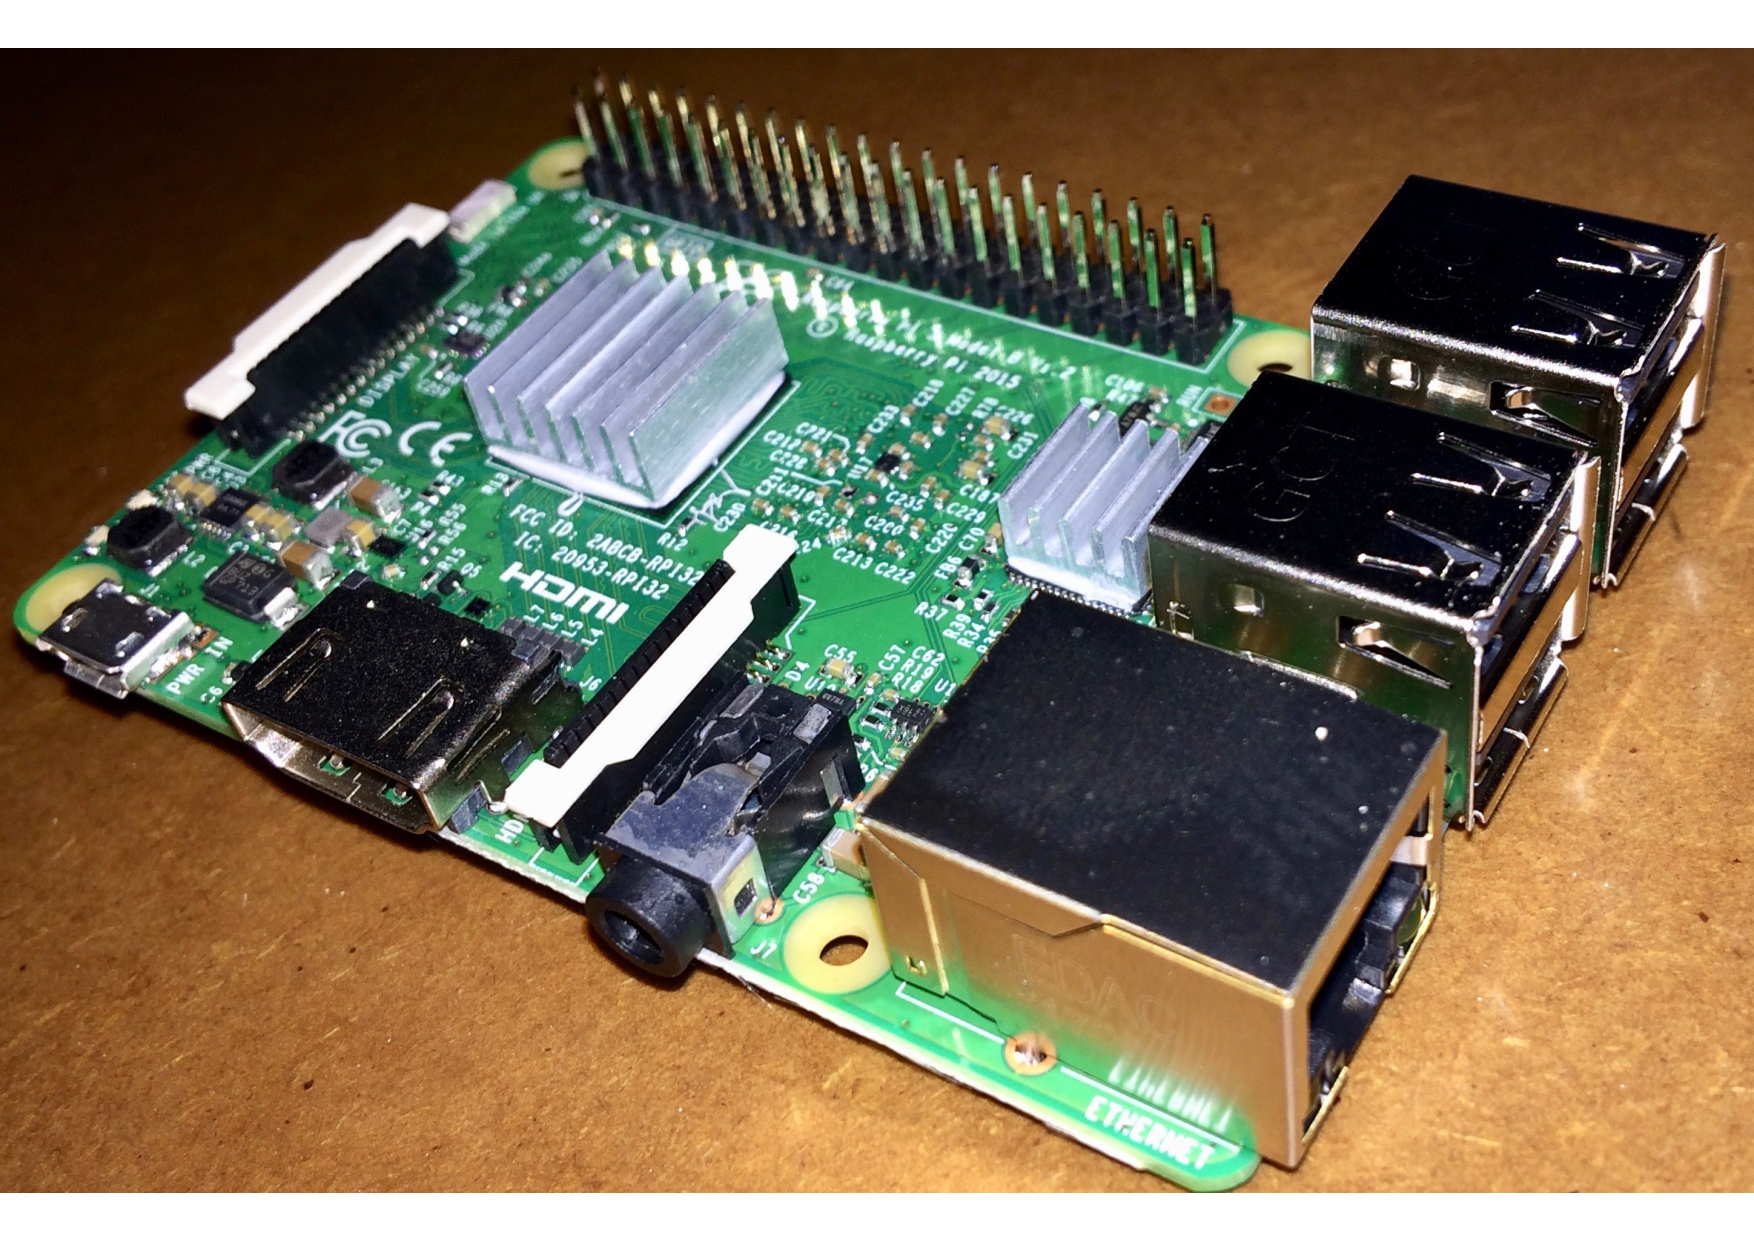
\includegraphics[width=0.9\textwidth]{raspi}
	\caption{Raspberry Pi 3.}\label{fig:raspi3b}
\end{figure}

Una vez descargado el sistema, este ha sido instalado en una micro SD mediante el siguiente procedimiento por consola\footnote{Realizado en OSX, aunque en Linux es muy similar}:
\begin{itemize}
\item\code{diskutil list} Permite localizar el dispositivo en el que se encuentra la tarjeta. En nuestro caso \code{/dev/disk4}
\item\code{diskutil umountDisk /dev/disk4} Permite desmontar el volumen. 
\item\code{sudo dd if=raspbian-stretch.img of=/dev/rdisk4 bs=1m} El comando \code{dd} copia la entrada estándar a la salida estándar. Mediante \code{if/of} se establece el fichero de entrada/salida. Mediante \code{bs} se establece el tamaño de bloque a copiar. Se está utilizando \code{/dev/\underline{\textbf{r}}disk4} en lugar de \code{/dev/disk4} debido a la capacidad de OSX de trabajar con dispositivos en bruto, \textit{raw}, de forma que es posible acceder al dispositivo de forma directa\footnote{Véase \code{man hdiutil}, sección \textit{DEVICE SPECIAL FILES}}, sin almacenar en un buffer la lectura del archivo, proporcionando velocidades de escritura/lectura hasta 20 veces más rápidas.
\end{itemize}


Una vez realizados estos pasos, se puede insertar la microSD en la Raspberry Pi. Para encenderla basta con utilizar el puerto micro-usb de que dispone.\\La Raspberry Pi 3 requiere de una fuente de alimentación capaz de proporcionar 2,5A\footnote{Véase https://www.raspberrypi.org/help/faqs/\#power} para funcionar al máximo nivel de estrés para el procesador y alimentar dispositivos USB.

Sin embargo, este no es estrictamente nuestro caso, véase el apartado \hyperref[subsec:Modificaciones]{Modificaciones}. Se requiere un dispositivo cuyo consumo sea lo más reducido posible, pero que sea rápido en la ejecución, y que muestre poca latencia en operaciones de \code{IO}, que es donde se encuentra el cuello de botella.

Una vez encendida, se accede a ella con el usuario por defecto \code{pi} y la contraseña por defecto \code{raspberry}. Obviamente ambas \textbf{han sido cambiadas} por motivos de seguridad.



\subsubsection{Modificaciones}
\label{subsec:Modificaciones}

\begin{figure}
	\centering
	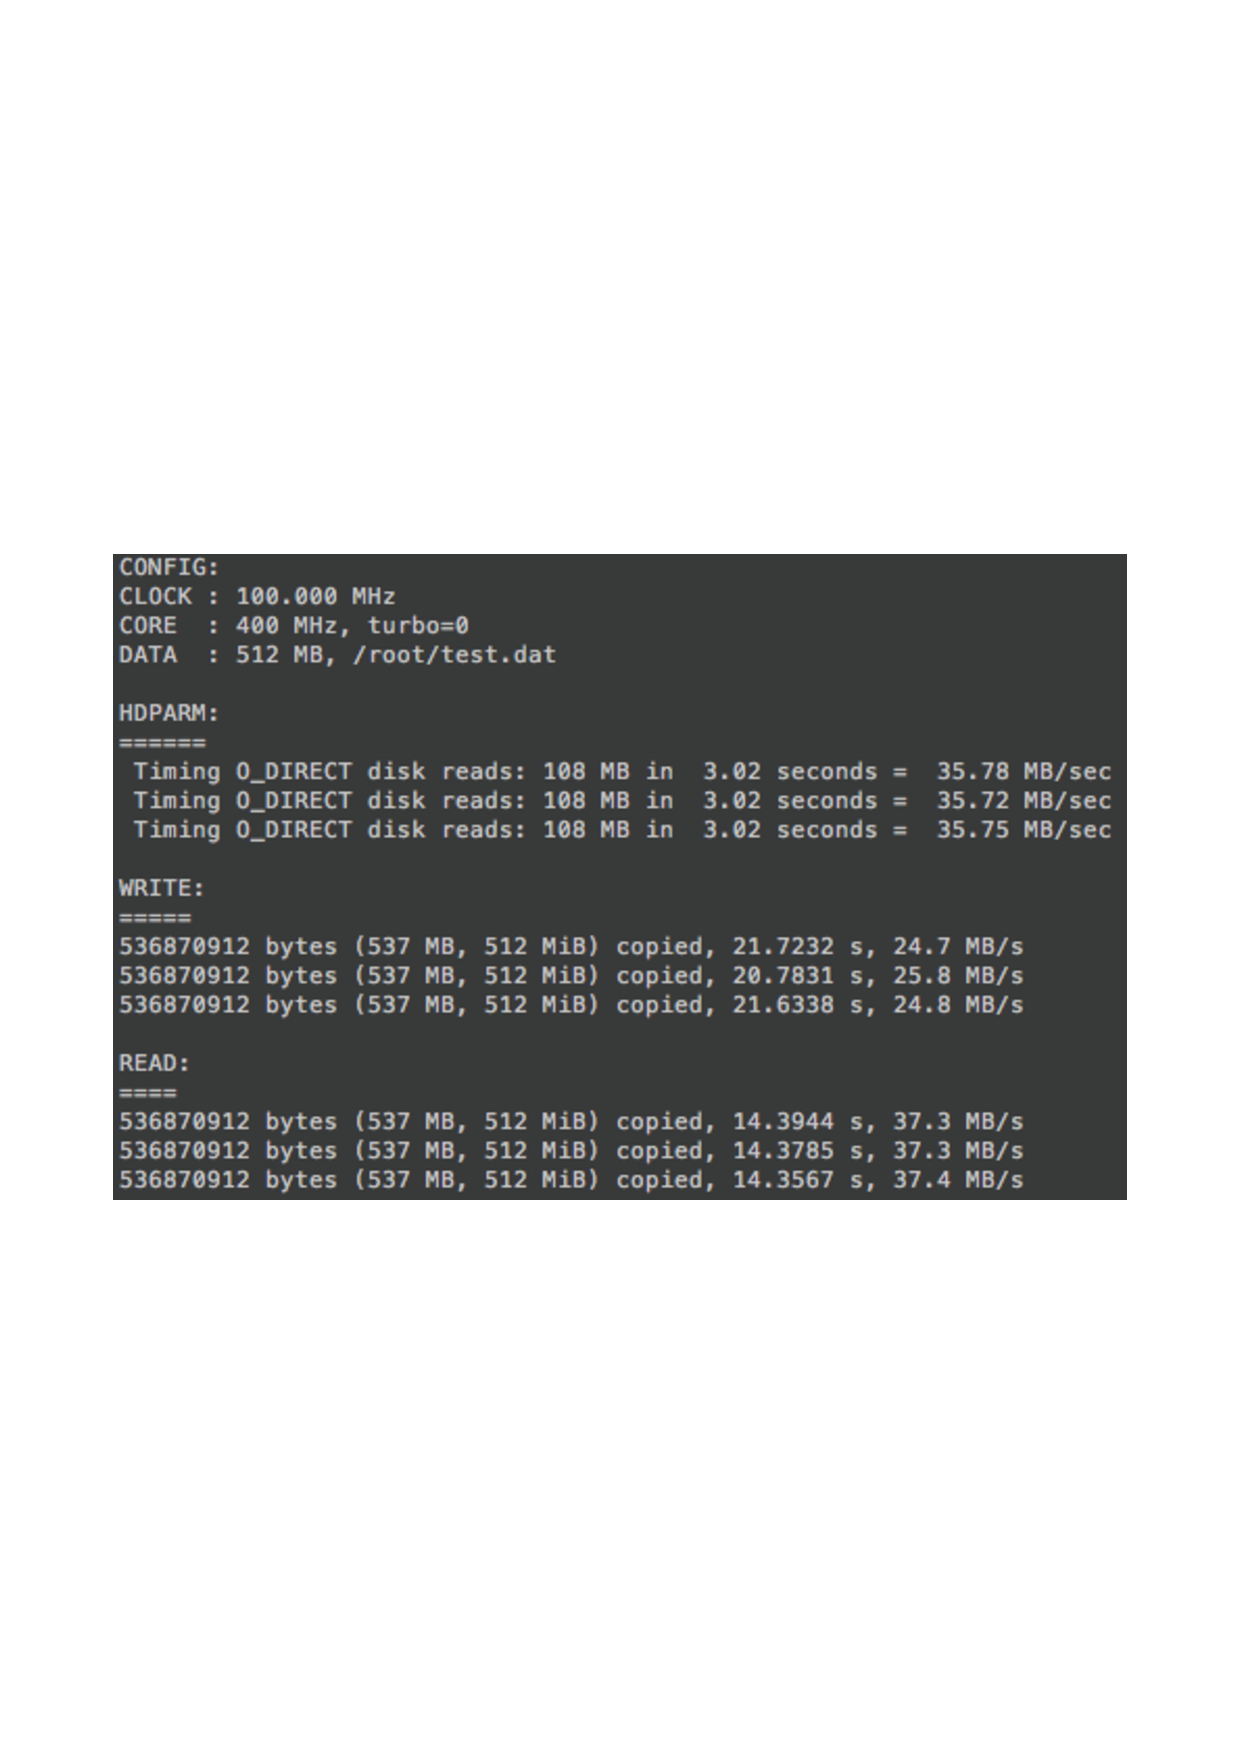
\includegraphics[width=0.9\textwidth]{sdbench}
	\caption{Benchmark de lector microSD OC.}\label{fig:sdbenchmark}
\end{figure}

\begin{itemize}
\item Se ha desactivado el puerto HDMI para reducir el consumo en \textasciitilde{}30mA: \\Para ello se ha incluido en \code{/etc/rc.local} la línea \code{/usr/bin/tvservice -o}.
\item Se ha overclockeado el lector de microSD a 100MHz, en lugar de los 50MHz por defecto: \\Para ello se ha incluido en \code{/boot/config.txt} la línea \code{dtparam=sd\_overclock=100}.\\Y que arroja los resultados mostrados en la imagen \ref{fig:sdbenchmark}
\item Se han incluido una serie de disipadores para evitar sobrecalentamiento de la placa. Así como un pequeño ventilador de bajo consumo.
\end{itemize} 




\section{Protocolos}

\subsection{MultiWii Serial Protocol}

\noindent Conocido como \textit{MSP}, se trata de un protocolo para la transferencia de información desde, o hacia una controladora de vuelo\footnote{Una controladora de vuelo es una pequeña placa electrónica que contiene un procesador, una serie de sensores (como acelerómetro, giroscopio, barómetro o magnetómetro) así como entradas y salidas, y que se encarga del control de estabilidad del drone.}.\\\\Generalmente es utilizado durante la configuración de la controladora de vuelo, para transmitir y recibir información de ella.
\\En el caso de este proyecto, se hará uso de este protocolo dado que existe la posibilidad de establecer la recepción de los canales de radio a través de un puerto serie. Es decir, en lugar de utilizar un receptor de radio, se utilizará un puerto serie para obtener la telemetría\footnote{La telemetría es el sistema de medición de magnitudes a distancia; i.e, transmite la información de los diferentes sensores de la controladora de vuelo. }, y establecer las entradas de los canales de radio.


\section{Referencias}

Las referencias se incluyen en el texto usando cite \cite{wiki:latex}. Para citar webs, artículos o libros \cite{koza92}.


\section{Imágenes}

Se pueden incluir imágenes con los comandos standard de \LaTeX, pero esta plantilla dispone de comandos propios como por ejemplo el siguiente:

\imagen{escudoInfor}{Autómata para una expresión vacía}



\section{Listas de items}

Existen tres posibilidades:

\begin{itemize}
	\item primer item.
	\item segundo item.
\end{itemize}

\begin{enumerate}
	\item primer item.
	\item segundo item.
\end{enumerate}

\begin{description}
	\item[Primer item] más información sobre el primer item.
	\item[Segundo item] más información sobre el segundo item.
\end{description}
	
\begin{itemize}
\item 
\end{itemize}

\section{Tablas}

Igualmente se pueden usar los comandos específicos de \LaTeX o bien usar alguno de los comandos de la plantilla.

\tablaSmall{Herramientas y tecnologías utilizadas en cada parte del proyecto}{l c c c c}{herramientasportipodeuso}
{ \multicolumn{1}{l}{Herramientas} & App AngularJS & API REST & BD & Memoria \\}{ 
HTML5 & X & & &\\
CSS3 & X & & &\\
BOOTSTRAP & X & & &\\
JavaScript & X & & &\\
AngularJS & X & & &\\
Bower & X & & &\\
PHP & & X & &\\
Karma + Jasmine & X & & &\\
Slim framework & & X & &\\
Idiorm & & X & &\\
Composer & & X & &\\
JSON & X & X & &\\
PhpStorm & X & X & &\\
MySQL & & & X &\\
PhpMyAdmin & & & X &\\
Git + BitBucket & X & X & X & X\\
Mik\TeX{} & & & & X\\
\TeX{}Maker & & & & X\\
Astah & & & & X\\
Balsamiq Mockups & X & & &\\
VersionOne & X & X & X & X\\
} 
